\section{RQ1. What do Gists look like?}

\subsection{Users and Their Gists}

As Table \ref{tb:userdistribution} shows, among the randomly sampled 562,993 GitHub users, only 32,786 (5.82\%) of them had at least one public Gist. 

\begin{table}[!htb]
 \begin{center}
 \begin{tabular}{@{}lrr} 
    \textbf{Users} &   \textbf{Count}        &  \textbf{Percentage} \\ \hline
    Users having at least one public Gist      &   32,786                 &   5.82\%             \\ 
    Users having no public Gists               &   530,207                &   94.18\%             \\ \hline
 \end{tabular}
 \end{center}
 \caption{Comparison of GitHub users having at least one public Gist and those having not any.}
 \label{tb:userdistribution}
\end{table}

For those 32,786 users having at least one public Gist, Figure \ref{fig:gistproportion} shows their distribution by the number of Gists per user. We can see that majority of users just have a small number of Gists. Specifically, 50\% of the users have less than 5 public Gists. 70\% have less than 10 public Gists. Only 4\% of users have 30 or more public Gists.

\begin{figure}[!htb]
	\centering
	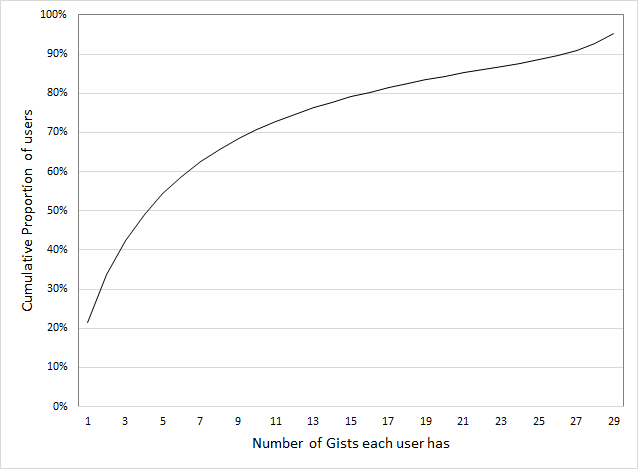
\includegraphics[width=0.8\textwidth]{figures/GistProportion.png}
	\caption{Users distribution by the number of Gists owned.}
	\label{fig:gistproportion}
\end{figure}

\subsection{Contents of Gists}
The content of Gists can be analyzed in several different aspects, such as the number of files per Gist, the languages, the MIME type, the size. All the analysis results in this section are against the sampled 618,393 Gists or the 793,891 files in those Gists.

\subsubsection{Number of Files per Gist}

GitHub doesn't restrain the number of files in each Gist. Table \ref{tb:files} shows the distribution of all sampled Gists based on the number of files they contain. It shows that majority of Gists (86.79\%) contain only one file. 

\begin{table}[!htb]
 \begin{center}
 \begin{tabular}{@{}rr} 
    \textbf{Number of Files Each Gist contains}	&	\textbf{Percentage of Gists} \\ \hline
	0	&	0.02\%\\
	1	&	86.79\%\\
	2	&	7.16\%\\
	3	&	3.16\%\\
	4	&	1.53\%\\
	$\geq$ 5	&	1.35\%\\\hline
 \end{tabular}
 \end{center}
 \caption{Distribution of Gists by number of files contained.}
 \label{tb:files}
\end{table}

It is expected that majority of Gists contain only a few files, since Gists are supposed to record and share small code snippets. However, one surprising observation was that there also existed Gists containing a lot of files (1001 files in a Gist at most). 

\subsubsection{Gist Files Types}
I analyzed the types of Gist files by their MIME types and their languages.

Figure \ref{fig:typeDist} shows the distribution of top 20 MIME types of all Gist files (there are other 93 falling into the ``Others'' category which is 0.4\%). It's obvious that text/plain dominates with 53.5\% which actually includes a variety of file types. Some programming languages are very common indicated by the MIME type, such as application/javascript (9.7\%), application/x-ruby (9.4\%), application/python (5.6\%), but we need to note that lots of programming languages fall into the text/plain category. Other common types include images (png 0.5\%, gif 0.4\%, jpeg 0.1\%), markup language text (html 3.7\%, xml 1.4\%, yaml 0.5\%), JSON data (1.7\%), etc. 

\begin{figure}[!htbp]
	\centering
	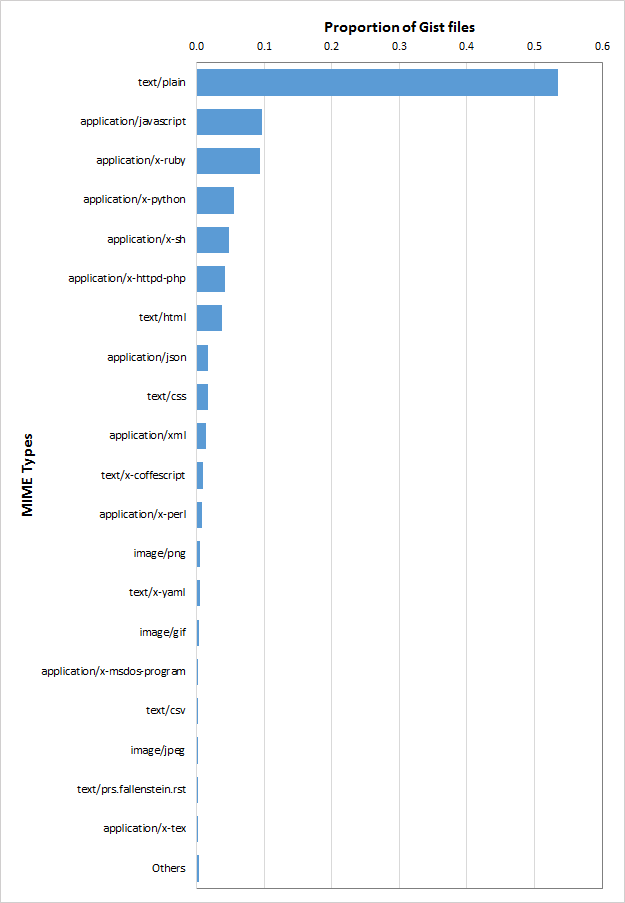
\includegraphics[width=0.8\textwidth]{figures/typeDistribution.png}
	\caption{Distribution of Gist files by MIME types.}
	\label{fig:typeDist}
\end{figure}

The Gist file metadata provides the language attribute for each file. 257 languages were discovered in total from our sample. Figure \ref{fig:languageDist} shows the distribution of top 30. We can see 27.9\% of Gist files don't have any languages. The most popular programming languages are Ruby (10.2\%), JavaScript (9.7\%), Python (5.6\%), Shell script (5.3\%). Lots of markup languages are very common too, which includes Markdown (4.6\%), HTML (3.7\%), JSON (1.9\%), XML (1.5\%), Diff (1.3\%). The ``Others'' category represents the other 227 languages that are not shown in the chart and they account for 5.8\%. 

\begin{figure}[!htbp]
	\centering
	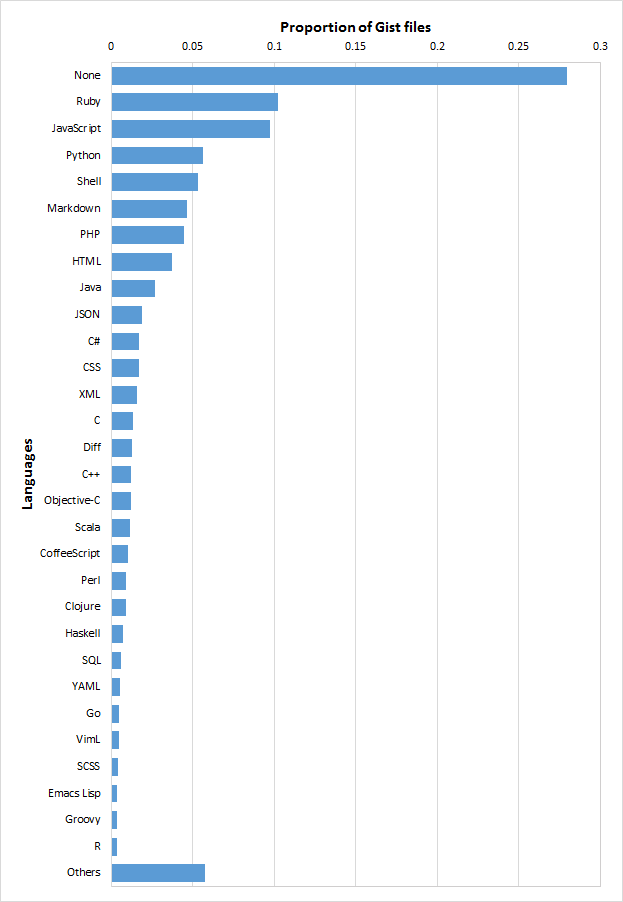
\includegraphics[width=0.8\textwidth]{figures/languageDistribution.png}
	\caption{Distribution of Gist files by language.}
	\label{fig:languageDist}
\end{figure}

\subsubsection{Size of Gist Files}
As for the size of Gist files, I looked into three metrics: size in bytes, number of lines for files of text or application MIME type, and SLOCs for source files. 

Figure \ref{fig:size} shows the distribution of Gist files in terms of their size in bytes. We can see majority of Gist files are around 1KB. The median value is 714 Bytes (quartiles are 287 and 1830 bytes). There exist outliers though: 0.17\% of Gist files are over 1MB.

\begin{figure}[!htb]
	\centering
	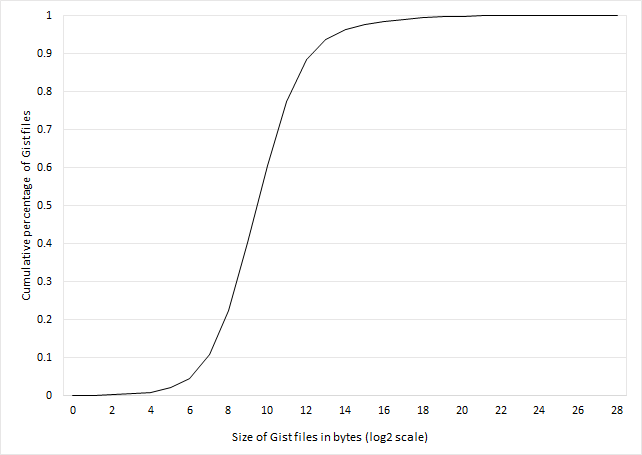
\includegraphics[width=0.8\textwidth]{figures/gist_file_size_log.png}
	\caption{Distribution of Gist files by size.}
	\label{fig:size}
\end{figure}

We also counted the number of lines for all the text files (783,326 in total). Figure \ref{fig:textlines} shows the distribution of these files by their number of lines. 87.1\% of them have less than 100 lines. The median value is 23 lines (quartiles are 10 and 55 lines).

\begin{figure}[!htb]
	\centering
	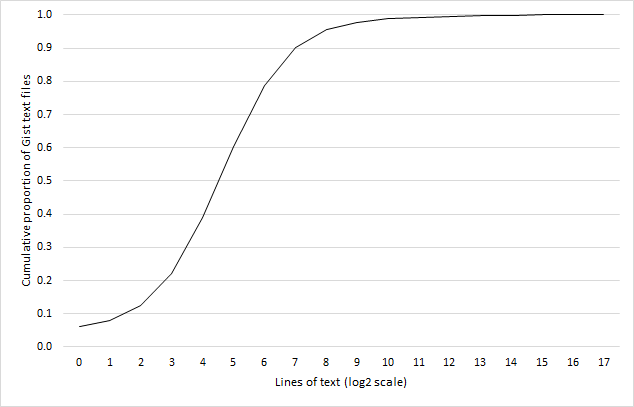
\includegraphics[width=0.8\textwidth]{figures/text_files_lines.png}
	\caption{Distribution of Gist text files by number of lines.}
	\label{fig:textlines}
\end{figure}

I ran \textit{CLOC} script against all Gist files to calculate their SLOC (binary or empty files would be ignored by \textit{CLOC}). \textit{CLOC} recognizes a source file by its extension or its first line of code. If the file does not have a recognized extension or is not a recognized scripting language, it would be ignored.\footnote{\url{https://github.com/AlDanial/cloc\#How_it_works}}. Finally 778,806 text files (98.1\% of all Gist files) were detected, from which 502,242 source files (64.5\% of all Gist text files, 63.3\% of all Gist files) were recognized as Table \ref{tb:clocfiles} shows. The distribution of source files by SLOC as is shown in Figure \ref{fig:sloc}. 54.8\% of them have less than 20 SLOCs, and 92.1\% have less than 100. The median value is 18 SLOCs (quartiles are 8 and 39 SLOCs).

\begin{table}[!htb]
 \begin{center}
 \begin{tabular}{@{}lr} 
    \textbf{Files}	&	\textbf{Count} \\ \hline
	All files of 618,393 Gists downloaded &	793,891\\
	--- Gist text files	&	778,806\\
	-------- Gist source files &	502,242\\ \hline
 \end{tabular}
 \end{center}
 \caption{Gist files recognized by CLOC}
 \label{tb:clocfiles}
\end{table}

\begin{figure}[!htb]
	\centering
	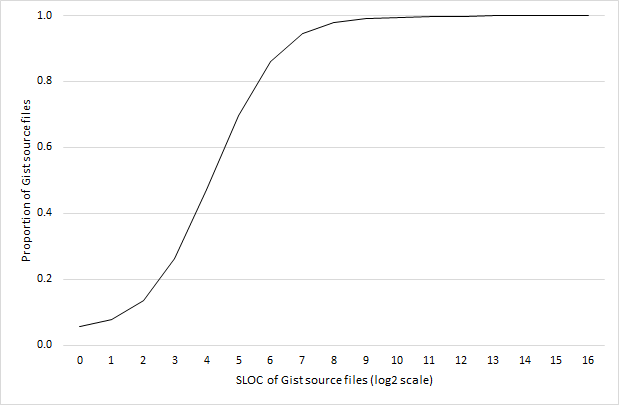
\includegraphics[width=0.8\textwidth]{figures/sloc.png}
	\caption{Distribution of Gist source files by SLOC.}
	\label{fig:sloc}
\end{figure}

\subsubsection{Uniqueness of Gist Files}
\textit{CLOC} is able to detect uniqueness for text files based on \textit{Digest:MD5}\footnote{\url{https://github.com/gisle/digest-md5}}. By taking advantage of that, I performed duplicate detection against all Gist files. Since \textit{CLOC} cannot detect duplicates for binary files, it only analyzed all the 778,806 text files from which 759,586 (97.5\% of all text files) files were detected as unique. It means that 2.5\% of text Gist files were duplicates.

\subsection{Activity}
Since Gists are like a GitHub repositories, we can trace users' activities against them, such as number of commits, number of comments, times of being forked, etc. As Figure \ref{fig:commits} shows, 62.9\% of Gists had a single commit. 32.1\% had 2 to 5 commits, and only 1.85\% of Gists had more than 10 commits. This result is also verified by the distribution of days between the creation the latest update for each Gist, which is shown in Figure \ref{fig:days}. We can see the creation and the latest update of 83.7\% of Gists happened at the same day. 

\begin{figure}[!htb]
	\centering
	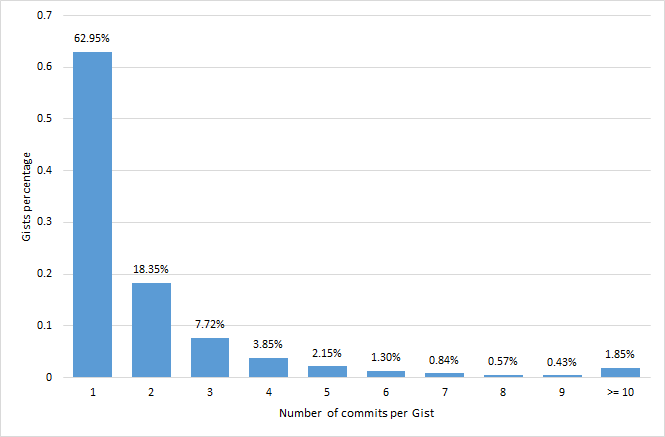
\includegraphics[width=0.8\textwidth]{figures/commits.png}
	\caption{Distribution of Gists by number of commits.}
	\label{fig:commits}
\end{figure}
\begin{figure}[!htb]
	\centering
	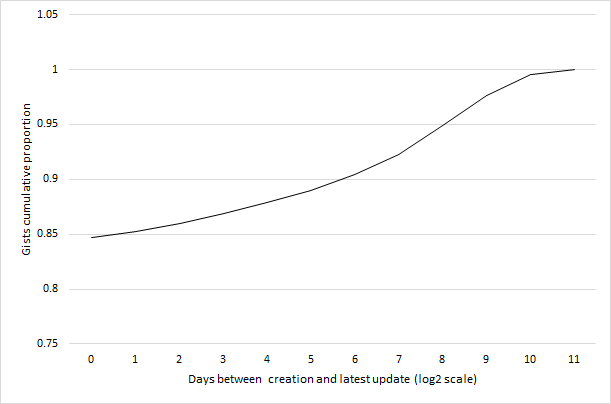
\includegraphics[width=0.8\textwidth]{figures/date_diff.png}
	\caption{Distribution of of Gists by days between creation and latest update.}
	\label{fig:days}
\end{figure}

In terms of forks, 94.6\% of Gists have never been forked, and 4.0\% of Gists have only been forked once. Only 0.7\% of Gists have been forked more than 3 times (shown in Table \ref{tb:forks}). Table \ref{tb:comments} shows the distribution of comments per Gist, from which we can see only 7.3\% of Gists have been commented once or more. All of these observations show that majority of Gists are not active.

\begin{table}[!htb]
 \begin{center}
 \begin{tabular}{@{}rr} 
    \textbf{Number of forks} &   \textbf{Gists proportion}\\ \hline
    0 &   94.6\% \\ 
    1 &   4.0\% \\ 
    2 &   0.7\% \\ 
    $\geq$ 3 &   0.7\%\\ \hline
 \end{tabular}
 \end{center}
 \caption{Distribution of Gists by number of forks.}
 \label{tb:forks}
\end{table}

\begin{table}[!htb]
 \begin{center}
 \begin{tabular}{@{}rr} 
    \textbf{Number of comments} &   \textbf{Gists proportion}\\ \hline
    0 &   92.7\% \\ 
    1 &   4.6\% \\ 
    2 &   1.3\% \\ 
    3 &   0.5\% \\ 
    $\geq$ 4 &   1.0\%\\ \hline
 \end{tabular}
 \end{center}
 \caption{Distribution of Gists by number of comments.}
 \label{tb:comments}
\end{table}

\subsection{Manual Inspection of Gists Content}

I manually inspected 400 randomly sampled Gists by assigning non-exclusive labels to each of them based on two aspects: the content of a Gist as a whole, and the relationships between files within a Gist. 

\subsubsection{Gists Content}
During categorizing these 400 Gists based on content with the labels shown in Table \ref{tb:gistcontentlabels}, It was observed that the contents of Gists were usually very short and demonstrated a big variety of uses. Code is expectedly the most dominant use, but I also found lots of other uses, such as blogs, configuration information, logs, data, letters, or even a restaurant menu. I also found Gist written in several other languages besides English. Moreover, I observed that the MIME type or language of a Gist file might not be enough to understand a Gist. For example, source code and plain text are often mixed together.

The result of categorizing is shown in Table \ref{tb:labels}. Note that the sum of all labels are more than 100\% because a Gist can be assigned several labels. It's not surprising that most of Gists (79.25\%) contain code, including complete programs, functions, code fragments, classes, test code. However, other types of Gists content cannot be dismissed: Log (7.5\%), Blog (1.5\%), Non-technical (1.5\%), etc.

\begin{table}[!htb]
 \begin{center}
 \begin{tabular}{@{}lr} \hline
    \textbf{Labels in terms of content}	&	\textbf{Percentage of Gists} \\ \hline
	Code & 79.25\%\\
	Note & 24.5\%\\
	Function & 10.0\%\\
	Log & 7.5\%\\
	Class & 6.5\%\\
	Data & 5.25\%\\
	Fragment & 4.75\%\\
	Command & 4.75\%\\
	Template & 4.0\%\\
	Test & 3.25\%\\
	Configuration & 3.25\%\\
	Diff & 1.75\%\\
	Blog & 1.5\%\\
	Non-technical & 1.5\%\\
	Documentation & 0.5\%\\
	Empty & 0.5\%\\ \hline
 \end{tabular}
 \end{center}
 \caption{Distribution of Gists by content labels.}
 \label{tb:labels}
\end{table}

\subsubsection{Files Relationships Within One Gist}
A Gist can have more than one file. When a Gist has multiple files, I observed that they were usually related. The 400 Gists were categorized with labels shown in Table \ref{tb:gistfilerelationshiplabels} to show the relationships between the files within each Gist, and the result is shown in Table \ref{tb:relationship}. We can see most Gists contained only one file. For those having multiple files, they spread approximately uniformly among different categories. Only 3.25\% of Gists have multiple files that are not related to each other. 

\begin{table}[!htb]
 \begin{center}
 \begin{tabular}{lr}
    \textbf{Relationship between files of each Gist}	&	\textbf{Percentage} \\ \hline
	Single File & 87.25\%\\
	Reference & 4.25\%\\
	Generation & 3.25\%\\
	Independent & 3.25\%\\
	Test & 1.25\%\\
	Attachment & 0.75\%\\ \hline
 \end{tabular}
 \end{center}
 \caption{Distribution of Gists by relationships between files}
 \label{tb:relationship}
\end{table}